%%%%%%%%%%%%%%%%%%%%%%%%%%%%%%%%%%%%%%%%%%%%%%%%%%%%%%%%%%%%%%%%%%%%%%%%%
% latex multiGrid
% xdvi multiGrid &
% dvips -D600 multiGrid.dvi -o multiGrid.ps
%%%%%%%%%%%%%%%%%%%%%%%%%%%%%%%%%%%%%%%%%%%%%%%%%%%%%%%%%%%%%%%%%%%%%%%%%
\documentclass[11pt]{article}
\usepackage{graphicx}
\usepackage{fullpage}
\usepackage{times}
\newcommand{\ProtoMol}{\textsc{ProtoMol }}
\author{Thierry Matthey\\{\tt matthey@ii.uib.no}}

\title{Multigrid}
%%%%%%%%%%%%%%%%%%%%%%%%%%%%%%%%%%%%%%%%%%%%%%%%%%%%%%%%%%%%%%%%%%%%%%%%%
\begin{document}
%%%%%%%%%%%%%%%%%%%%%%%%%%%%%%%%%%%%%%%%%%%%%%%%%%%%%%%%%%%%%%%%%%%%%%%%%
\maketitle
%%%%%%%%%%%%%%%%%%%%%%%%%%%%%%%%%%%%%%%%%%%%%%%%%%%%%%%%%%%%%%%%%%%%%%%%%

%%%%%%%%%%%%%%%%%%%%%%%%%%%%%%%%%%%%%%%%%%%%%%%%%%%%%%%%%%%%%%%%%%%%%%%%%
\section{Introduction}

Multi grid is a method for the fast summation of long range forces,
i.e. Coulomb force, in a system consisting of a large number of
particles. For $N$-particle system, multi grid has a time complexity
of $O(N)$, where the direct solution, the Ewald Sum and Particle Mesh
Ewald are of order $O(N^2)$, $O(N^{\frac{3}{2}})$ respectively
$O(N\log N)$. Multi grid decomposes the Coulomb interaction between the
particles into a local and a smooth part.
\begin{figure}[htb]
  \centerline{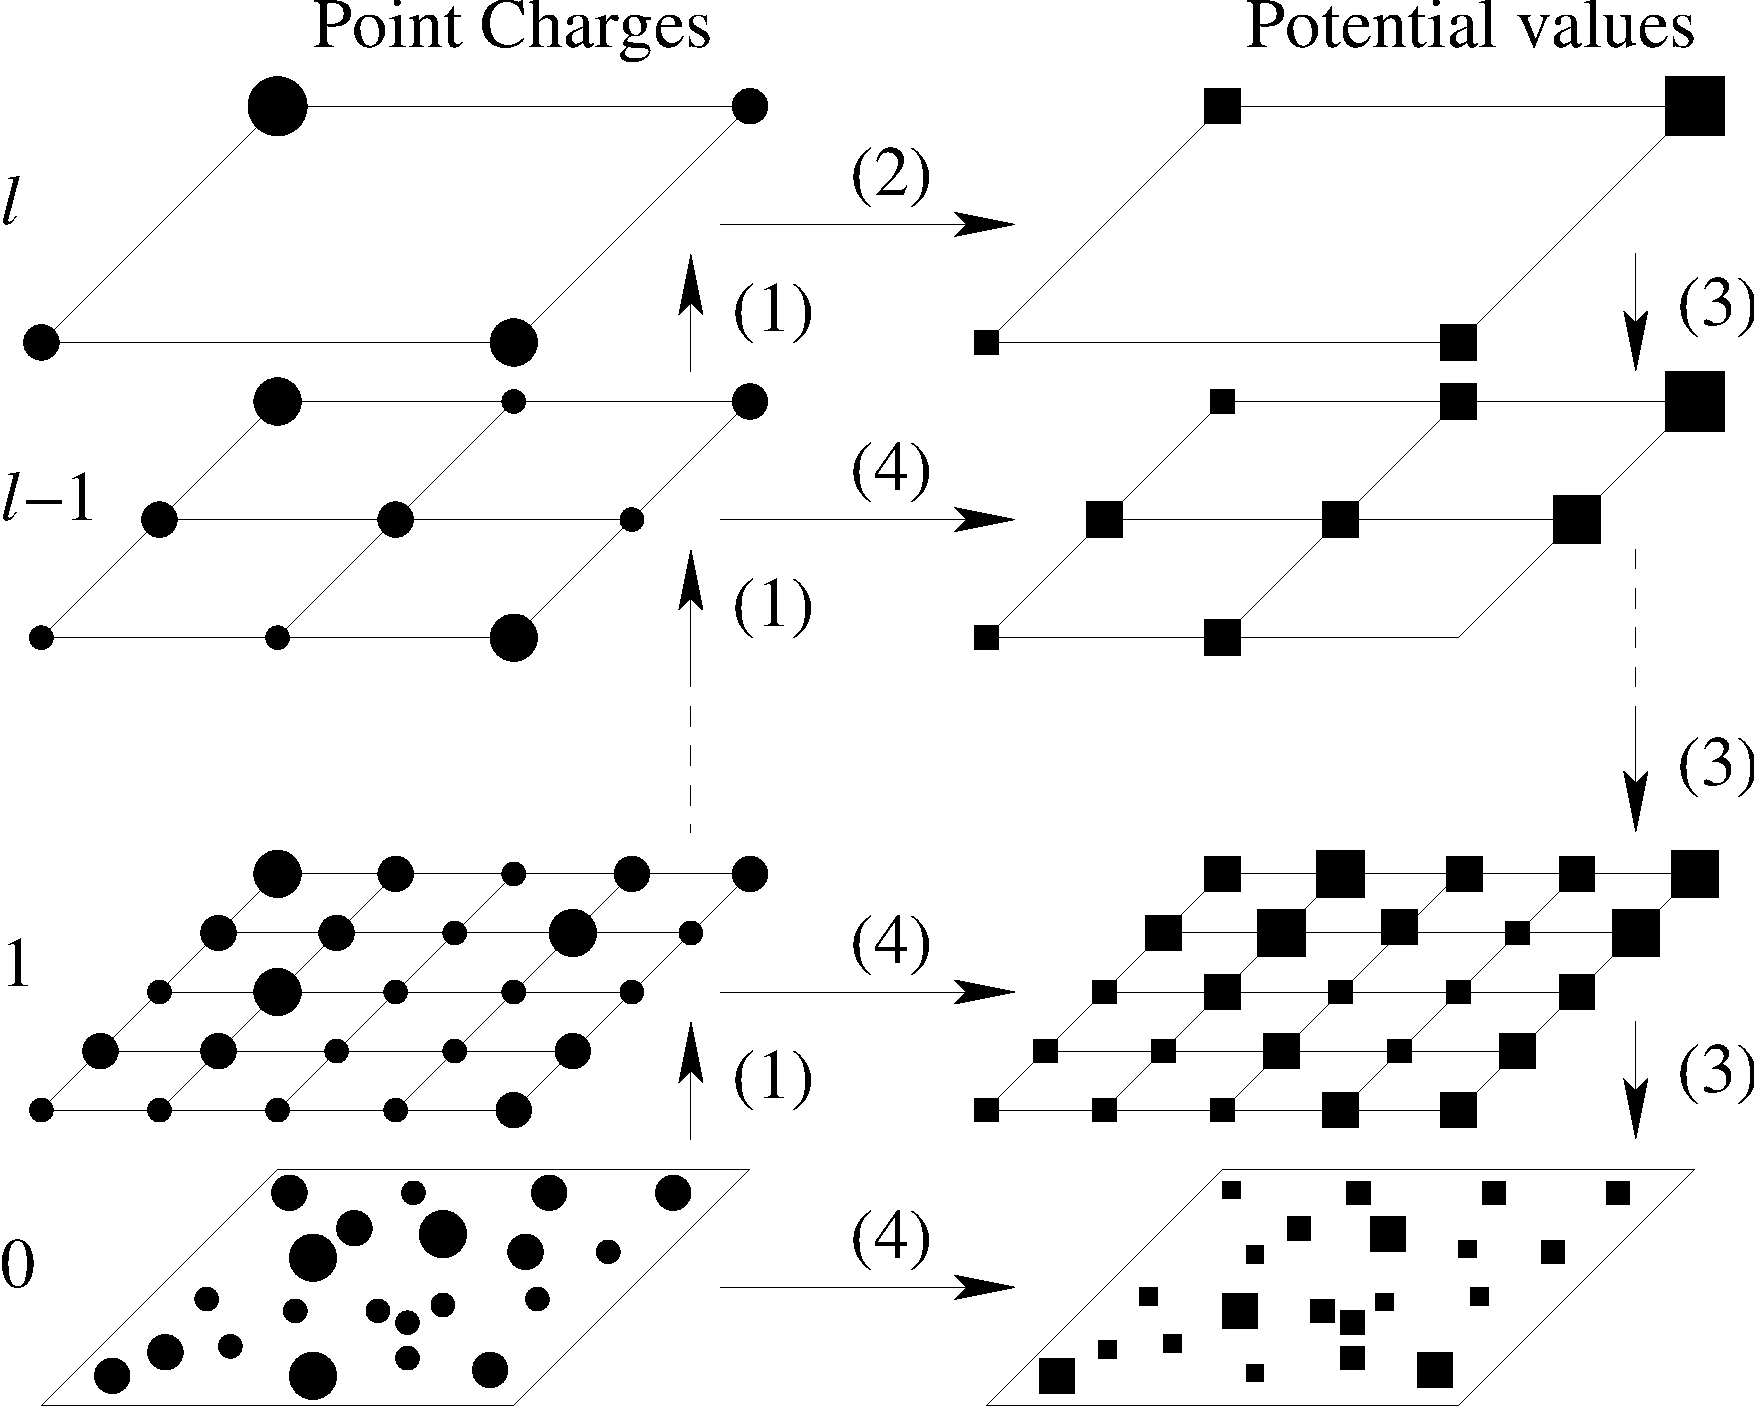
\includegraphics[width=10cm]{multigrid.pdf}}
  \caption[The multilevel scheme of the multi-grid algorithm.]{\small The
  multilevel scheme of the multi-grid algorithm. (1)
  Aggregate to coarser grids; (2) Compute potential induced by the
  coarsest grid; (3) Interpolate potential values from coarser grids;
  (4) Local corrections.\label{fig:multigrid}}
\end{figure}
\clearpage
%%%%%%%%%%%%%%%%%%%%%%%%%%%%%%%%%%%%%%%%%%%%%%%%%%%%%%%%%%%%%%%%%%%%%%%%%
\section{Input parameters}

This sections gives the definition of the multi grid input parameters
for \ProtoMol. 

%%%%%%%%%%%%%%%%%%%%%%%%%%%%%%%%%%%%%%%%%%%%%%%%%%%%%%%%%%%%%%%%%%%%%%%%%
\subsection{General syntax}

\ProtoMol\  expects the following input for multi grid:
\small
\begin{verbatim}
  -algorithm MultiGrid -interpolation <Hermite|BSpline> -kernel <C1|C2|C3|C4>
  -direct -smooth -correction
    -s            <real,positive>       
    -toplevelgrid <uint,positive> <uint,positive> <uint,positive> # PBC
    -h            <coordinates,non-zero>                          # Vacuum
    -origin       <coordinates=0 0 0>                             # Vacuum
    -levels       <int,positive>
    -order        <uint=4,positive>     
    -ratio        <uint=2,positive>
 \end{verbatim}
\normalsize
, where \texttt{=}{\it value} defines the default value, i.e. optional
input.\\
Note that \texttt{Coulomb} can be replaced by a new, user defined potential,
which is of the form $c r^a$, where $c$ is a constant and $r$ is the
distance between particle pairs. The new potential also requires
re-definition of \texttt{C1}, \texttt{C2},  \texttt{C3} and
\texttt{C4}. For the Lennard-Jones potential a new template is
required due to the sum in the potential definition.

%%%%%%%%%%%%%%%%%%%%%%%%%%%%%%%%%%%%%%%%%%%%%%%%%%%%%%%%%%%%%%%%%%%%%%%%%
\subsection{Interpolation}

\texttt{-interpolation} defines the interpolation scheme between the
grids the particle level. For the moment \ProtoMol\
does only accept Hermitian interpolation (\texttt{Hermite}). Other
interpolations like b-splines (\texttt{BSpline}) did not improve the
accuracy.

%%%%%%%%%%%%%%%%%%%%%%%%%%%%%%%%%%%%%%%%%%%%%%%%%%%%%%%%%%%%%%%%%%%%%%%%%
\subsection{Kernel}

\texttt{-kernel} defines how the {\it kernel} $G(r)$ (i.e. the Coulomb
potential, $r=|\vec{r}_{i} - \vec{r}_{j}|$)  is
{\it softened}. To {\it smooth} the kernel we only modify in a local range
$r<s$, where $s$ is the softening
distance. The {\it smoothed kernel} is defined as follow:
\begin{equation}
  G_{smooth}(r) \left\{
 \begin{array}{lcl}
  G_s(r) & : & r<s\\
  G(r)   & : & \mbox{otherwise}
 \end{array}
\right.
\end{equation}
, where $G_s(r)$ is the {\it smoothing function}. \texttt{C1},
\texttt{C2},  \texttt{C3} and  \texttt{C4} are smoothing functions
$G_s(r)$, which satisfy the the $C^1$, $C^3$, $C^3$ respectively
$C^4$ property. The smoothing  functions fit
only together with the Coulomb potential ($C\frac{q_i
  q_j}{|\vec{r}_{i} - \vec{r}_{j}|}$).

%%%%%%%%%%%%%%%%%%%%%%%%%%%%%%%%%%%%%%%%%%%%%%%%%%%%%%%%%%%%%%%%%%%%%%%%%
\subsection{Direct, smooth part and correction}

\texttt{-direct} \texttt{-smooth} and \texttt{-correction} indicate the part to be
 evaluated. \texttt{-correction} accounts the point self energy and the
 intra molecular term. By default (none of them set) all parts are computed. 


%%%%%%%%%%%%%%%%%%%%%%%%%%%%%%%%%%%%%%%%%%%%%%%%%%%%%%%%%%%%%%%%%%%%%%%%%
\subsection{S - softening distance}

\texttt{-s} defines the softening distance of the smoothed kernel
$G_{smooth}(r)$. It defines also the local correction at
each grid level. The softening distance is scaled according the ratio
and the actual level.
\\
An increased softening distance will increase the accuracy, but also
the computational work. A softening distance of order of the simulation
box results in a $O(N^2)$ time complexity. 

%%%%%%%%%%%%%%%%%%%%%%%%%%%%%%%%%%%%%%%%%%%%%%%%%%%%%%%%%%%%%%%%%%%%%%%%%
\subsection{Toplevelgrid and gridsize}

\texttt{-toplevelgrid} defines the number of grid points in each
dimension ($n_x$, $n_y$, $n_z$)  for the coarsest grid for vacuum systems, the one on the
top. \ProtoMol will
itself figure out the number of grid points required, for each finer
grid. \texttt{-h} defines the size (length, not grid points) of the finest
grid under PBC.\\
In case of periodic boundary conditions the relation of grid
points between to grids is defined by the ratio (\texttt{-ratio}) and
mesh size of the finest grid (\texttt{-g}):
\begin{equation}
  n_f = n_c \cdot \mbox{ ratio}
\end{equation}
Obviously, the length, depth and high of the grids are the same ($ d_f
= d_c$), defined by the cell basis vectors. The
number of grid points of the toplevel is equivalent to the number of
subdivision for the coarsest grid (Fig. \ref{fig:levels_bpc}).
\begin{figure}[hbt]
  \centerline{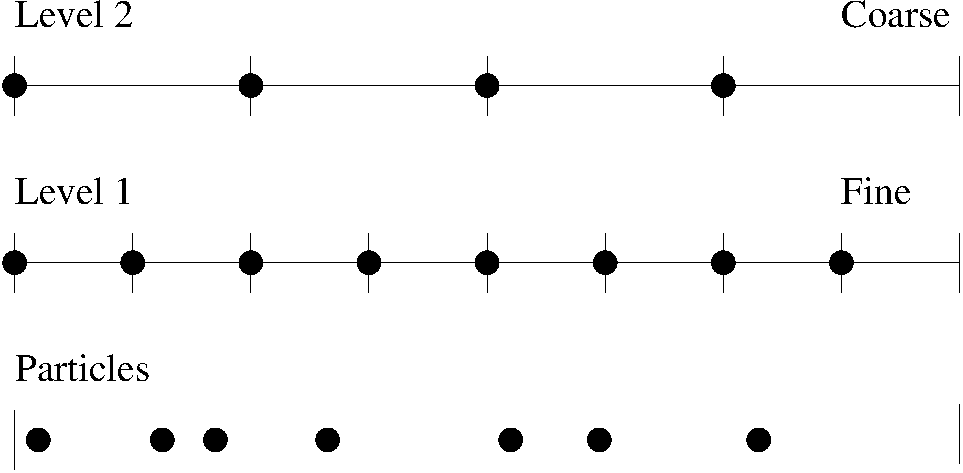
\includegraphics[width=3cm]{levels_pbc.pdf}}
  \caption{2-level, periodic boundaries, ratio, $n_1 = n_2 = 8$, $d_1 = d_2$, .}
  \label{fig:levels_bpc}
\end{figure}
\\
For the case of vacuum (i.e. no boundaries) the relation between two grids
and its dimensions depends on the ratio, the interpolation and order of interpolation:
\begin{equation}
  n_f = (n_c - \mbox{ order }+1) \mbox{ ratio } +1
\end{equation}
, assuming Hermitian interpolation, where for other interpolation
schemes the inner $+1$ may fall away. For the correctness of
interpolation the coarser grid must overlap the finer grid (Fig. \ref{fig:levels_nbc}). 
The length, depth and high of the finer grid is computed as follow:
\begin{equation}
  d_f = \frac{d_c n_f-1}{\mbox{ratio }(\mbox{order }-2)}
\end{equation}
, assuming Hermitian interpolation, where for other interpolation
schemes the $-2$ may change to $-1$.
\begin{figure}[hbt]
  \centerline{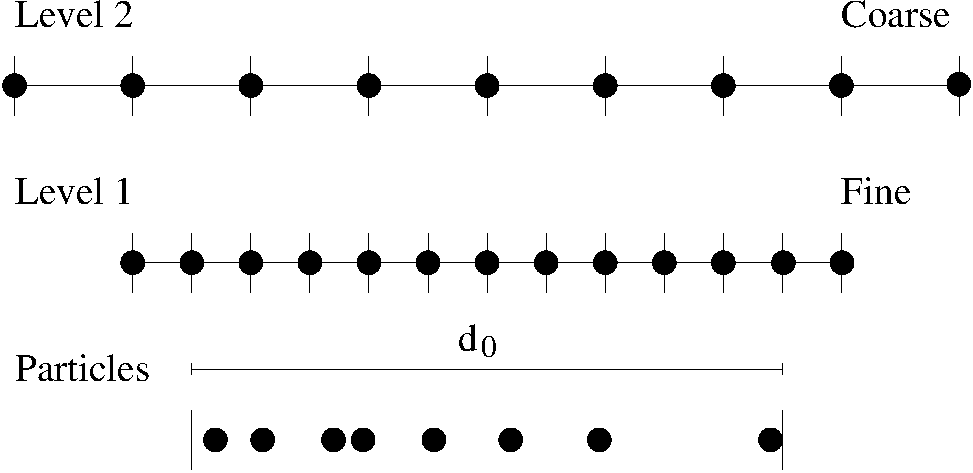
\includegraphics[width=3cm]{levels_nbc.pdf}}
  \caption{2-level, no boundaries, 4-order, ratio 2, $n_1 = 13$,
  $n_2 = 9$, $d_1 = \frac{6}{5}d_0$, $d_2 = \frac{8}{5}d_0$.}
  \label{fig:levels_nbc}
\end{figure}
\\
From experiments we see that the number of grid points in each
dimension for the coarsest grid  should be at least the double of the interpolation order,
this yields especially for vacuum. Further the
number of grid points for the finest grid should reflect a mesh size
of the order of the average distance between particles.


%%%%%%%%%%%%%%%%%%%%%%%%%%%%%%%%%%%%%%%%%%%%%%%%%%%%%%%%%%%%%%%%%%%%%%%%%
\subsection{Origin - optional, vacuum}
\texttt{-origin} defines the origin of the finest grid. It's optional
and only available for vacuum.


%%%%%%%%%%%%%%%%%%%%%%%%%%%%%%%%%%%%%%%%%%%%%%%%%%%%%%%%%%%%%%%%%%%%%%%%%
\subsection{Levels}

\texttt{-levels} defines the number of levels (grids).
\\
From experiments we know that finest grid should reflect a mesh size
of order of the average distance between particles. Note that the number of
levels and the ratio (\texttt{-ratio}) define roughly the relation of
grid points between the fines and the coarsest grid. The relation is of
 $\mbox{ratio}^{levels}$.

%%%%%%%%%%%%%%%%%%%%%%%%%%%%%%%%%%%%%%%%%%%%%%%%%%%%%%%%%%%%%%%%%%%%%%%%%
\subsection{Order - optional}

\texttt{-order} defines the interpolation order. The interpolation
order must be even, where 4 and 6 stand for a {\it cubic} and
{\it quintic} interpolation respectively.
\\
From experiments we see that the interpolation order and the smoothing
function $G_S(r)$ must correspond.

%%%%%%%%%%%%%%%%%%%%%%%%%%%%%%%%%%%%%%%%%%%%%%%%%%%%%%%%%%%%%%%%%%%%%%%%%
\subsection{Ratio}

\texttt{-ratio} defines the ratio of grid points between a fine and
coarse grid.
\\
Mostly 2 is used as ratio. For higher order interpolations a ratio
more than 2 may be an option.

%%%%%%%%%%%%%%%%%%%%%%%%%%%%%%%%%%%%%%%%%%%%%%%%%%%%%%%%%%%%%%%%%%%%%%%%%
\section{Optimization}

An efficient and equivalent definition of the force filed is compute the
direct part along with the Lennard-Jones. A separate definition for van
der Waals nonbonded interactions (LennardJones) and electrostatics and
be rewritten as following:\\~\\
\small
\begin{minipage}[htb]{6cm} 
\begin{verbatim}
# Only LennardJones by cutoff
force time LennardJones  
   -switchingFunction C2 
   -algorithm NonbondedCutoff
   -switchon 0.1
   -cutoff 10.0
# Only Coulomb bt multi grid
force time Coulomb 
   -algorithm MultiGrid 
   -interpolation Hermite 
   -kernel C3
   -levels 2
   -s 10
   -order 6
   -ratio 2
   -h 3 3 3
   -origin 0 0 0





\end{verbatim}
\end{minipage} 
\normalsize
 $\Rightarrow$ \,
\small
\begin{minipage}[htb]{12cm}
\begin{verbatim}
# LennardJones and direct part of multi grid
force time LennardJones CoulombMultiGridDirect 
    -kernel C3 
    -switchingFunction C2 
    -switchingFunction Cutoff 
    -algorithm NonbondedCutoff
    -switchon 0.1
    -cutoff 10.0
    -s 10
# Only smooth and correction part of multi grid
force time Coulomb 
    -algorithm MultiGrid 
    -interpolation Hermite 
    -kernel C3  
    -smooth 
    -correction
    -levels 2
    -s 10
    -order 6
    -ratio 2
    -h 3 3 3
    -origin 0 0 0
\end{verbatim}
\end{minipage}
\normalsize\\

One can expect speed up of 25\% or more with this equivalant
(mathematically) definition. Note that, one have to expect some
energy differences at some point, since the summation oder of forces
and energies has changed. Furthermore, one may consider to use a
look-up-table for the direct part of multi grid (i.e.,
\texttt{CoulombMultiGridDirectTable}). In most cases one will not
gain much performance, only with great loss of accuracy, i.e., small
look-up-table size (\texttt{-size}). In case of PME or plain Ewald,
this approach can improve performance with reasonable accuracy, since
the direct part of PME or plain Ewald is much more expensive than the
direct part of of multi grid.




%%%%%%%%%%%%%%%%%%%%%%%%%%%%%%%%%%%%%%%%%%%%%%%%%%%%%%%%%%%%%%%%%%%%%%%%%
\section{Compilation}

For experimental purpose the multi grid has several conditional compilation
flags.\\
\begin{tabular}{cp{7cm}}
\texttt{\small DEBUG\_MULTIGRID}         & Debug\\
\texttt{\small DEBUG\_MULTIGRID\_TIMING} & Printing the different timings\\
\end{tabular}

%%%%%%%%%%%%%%%%%%%%%%%%%%%%%%%%%%%%%%%%%%%%%%%%%%%%%%%%%%%%%%%%%%%%%%%%%
\end{document}
%%%%%%%%%%%%%%%%%%%%%%%%%%%%%%%%%%%%%%%%%%%%%%%%%%%%%%%%%%%%%%%%%%%%%%%%%
